\documentclass{standalone}
\usepackage{tikz}
\usepackage{pgfplots}
\pgfplotsset{compat=newest}
\usepackage{amsmath}
\usepackage[american]{circuitikz}
\usepackage{cmbright}

\definecolor{myred}{RGB}{170,0,0}
\definecolor{myblue}{RGB}{0,0,220}
\definecolor{mygreen}{RGB}{0,150,0}
\definecolor{myorange}{RGB}{255,127,0}
\definecolor{mybrown}{RGB}{150,75,0}

\begin{document}
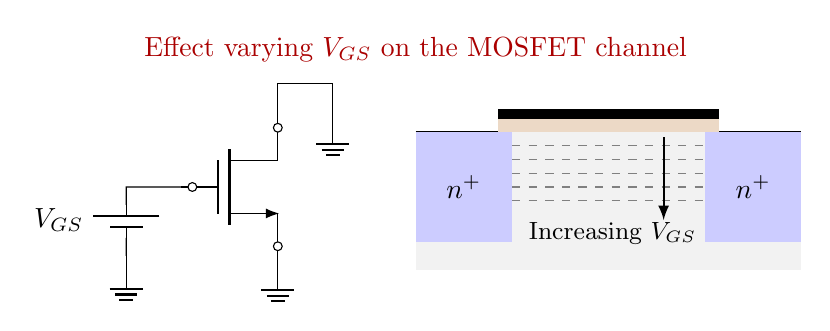
\begin{tikzpicture}
    \begin{scope}[scale=0.7]
        % Title
        \node[anchor=center, color=myred] at (2.5, 2.5) {Effect varying $V_{GS}$ on the MOSFET channel};
        
        % npn BJT sumbol
        \draw (0, 0) node[nmos, scale=1.25] (Q) {};
        \draw (Q.gate) 
            to ++(-1, 0)
            to[battery1, l_=$V_{GS}$] ++(0, -1.25)
            node[ground] {};
        \draw (Q.source)
            to ++(0, 0.1)
            node[ground] {};
        \draw (Q.drain)
            to ++(0, 0.5)
            to ++(1.0, 0)
            to ++(0, -0.5)
            node[ground] {};
        \draw[-Latex, thin] ($(Q.source) + (-0.6, 0.895)$) -- ++(0.625, 0);
        % Add the transistor nodes.
        \node[ocirc] at ($(Q.gate) + (0.2, 0)$) {};
        \node[ocirc] at ($(Q.source) + (0, 0.3)$) {};
        \node[ocirc] at ($(Q.collector) + (0, -0.3)$) {};

        % Show the MOSFET structure with the channel
        % Define an origin for depicting the MOSFET channel
        \node (O) at (6, 1) {};
        \node (W) at (3.5, 0) {};
        \node (WchBottom) at (0, 2.0) {};
        \node (WchTop) at (1.75, 0.0) {};
        \draw[thin, black] ($(O) - (W)$) -- ($(O) + (W)$);
        % Draw the p-type substrace
        \draw [fill=gray!10, draw=none] ($(O) - (W) - (0, 2.5)$) rectangle ($(O) + (W)$);
        % Draw the two n+ regions
        \draw [fill=blue!20, draw=none] ($(O) - (W) - (WchBottom)$) rectangle ($(O) - (W) + (WchTop)$);
        \draw [fill=blue!20, draw=none] ($(O) + (W) - (WchBottom)$) rectangle ($(O) + (W) - (WchTop)$);

        % Draw the gate
        \draw [fill=brown!30, draw=none] ($(O) + (-2.0, 0)$) rectangle ($(O) + (2.0, 0.25)$);
        \draw[thin, fill=black] ($(O) + (-2.0, 0.25)$) rectangle ($(O) + (2.0, 0.4)$);

        % Dotted lines depicting channels of different depths
        \draw[dashed, thin, black!50] ($(O) - (W) + (1.75, -0.25)$) -- ($(O) + (W) + (-1.75, -0.25)$);
        \draw[dashed, thin, black!50] ($(O) - (W) + (1.75, -0.5)$) -- ($(O) + (W) + (-1.75, -0.5)$);
        \draw[dashed, thin, black!50] ($(O) - (W) + (1.75, -0.75)$) -- ($(O) + (W) + (-1.75, -0.75)$);
        \draw[dashed, thin, black!50] ($(O) - (W) + (1.75, -1.00)$) -- ($(O) + (W) + (-1.75, -1.00)$);
        \draw[dashed, thin, black!50] ($(O) - (W) + (1.75, -1.25)$) -- ($(O) + (W) + (-1.75, -1.25)$);

        % n+ annotation
        \node[anchor=center, color=black] at ($(O) - (W) + (0.875, -1.00)$) {$n^+$};
        \node[anchor=center, color=black] at ($(O) + (W) + (-0.875, -1.00)$) {$n^+$};
        
        % Arrow indicating increasing channel depth
        \draw[-latex, thick, black] ($(O) + (1.0, -0.1)$) -- ($(O) + (1.0, -1.6)$);
        \node[xshift=-0.65cm, yshift=-0.0cm, color=black] at ($(O) + (1.0, -1.85)$) {\small Increasing $V_{GS}$};
    \end{scope}
\end{tikzpicture}
\end{document}